\section{Permission Bypassing Attack}
In this section, we demonstrate that it is possible for an adversary to  bypass requesting notification permission and successfully send push notifications to an end user.  For this attack to successfully work, we assume that attacker has control of a web page from a benign website  through exploits, phishing or other means. We will refer to the website as "benign.com" and the web page as "benign.com/attack" for further explanation. Let's say the website "benign.com" already provides push notification service to it's users (refer \ref{bypassAttack} step 1 ).If an user hasn't granted permission to "benign.com", then on visiting "bening.com/attack" page would be asked for permission as shown in step 2 of \ref{bypassAttack}. On the other hand, suppose there are users who have subscribed to notifications from "benign.com" as shown in step 3 of \ref{bypassAttack}.  In order for the adversary to take advantage of the notification permission that was already provided to the domain "benign.com", the only action required for the adversary to start sending notifications to the website's users is to register a service worker under domain "benign.com" on the users' machines. When an user visits the web page "benign.com/attack", the attacker's service worker would automatically get registered and the attacker is free to send any number of notifications to the user and all these notifications would appear to be sent by "benign.com" as shown in step 4 of \ref{bypassAttack}. In such a scenario, end user would blindly trust the notifications sent by the adversary and could be easily redirected to pages that may be used to obtain sensitive information from the user. This attack could also be used as a mean to make a website's users lose their trust in the website as they would be getting a lot of annoying or fake notifications. This attack is powerful than existing phishing attacks as even after web pages such as "benign.com/attack" is blacklisted, attacker would still be able to send notifications to the users who have already visited the page once. The only way to end the notifications would be for the user himself/herself to unregister the service worker of the attacker or revoke notification permission for the entire domain.

\begin{figure}[ht]
\caption{Demo of Bypass Notification Attack }
\begin{center}
\label{bypassAttack}
\begin{tabular}{cc}

 \begin{minipage}{.2\textwidth}
      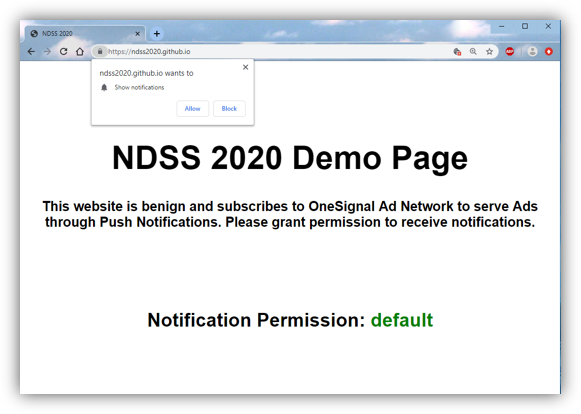
\includegraphics[width=\linewidth]{figs/attack_1.PNG}{1}
    \end{minipage}
 & 
\begin{minipage}{.2\textwidth}
      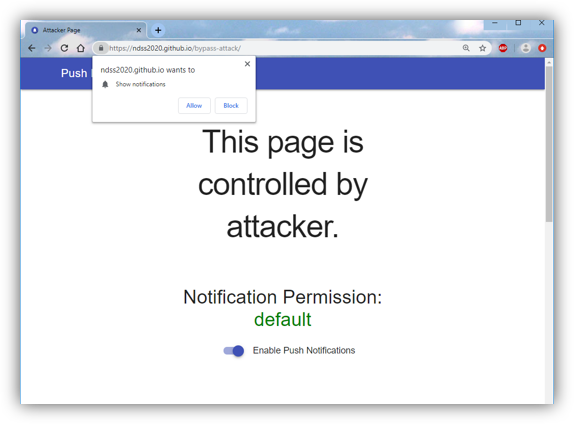
\includegraphics[width=\linewidth]{figs/attack_2.PNG}{2}
    \end{minipage}
 \\
 
\end{tabular}
      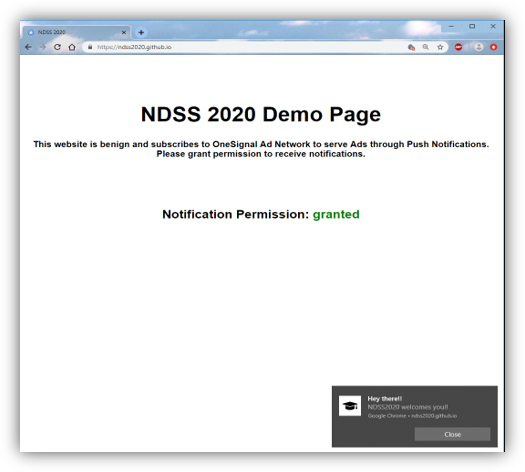
\includegraphics[width=\linewidth]{figs/attack_3.PNG}{3}
      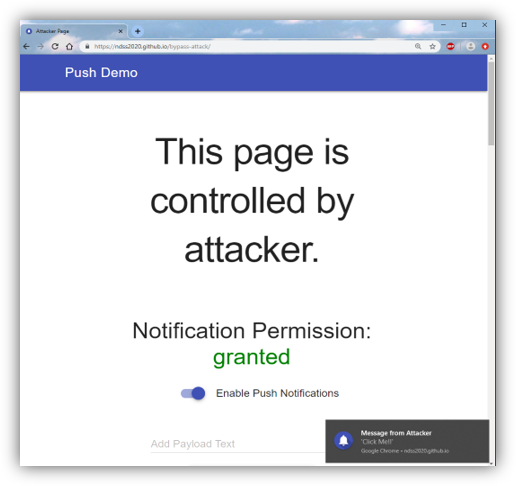
\includegraphics[width=\linewidth]{figs/attack_4.PNG}{4}
\begin{tabular}{c c}
\hline
\end{tabular}
\label{tab1}
\end{center}
\end{figure}
 

\noindent There are two main reasons for this attack to be possible. First, when an user grants permission, it is granted at the domain level and domain/website is blindly trusted. Second, any given website can register any number of service workers without user's permission as long as the multiple service workers are registered from different pages of the website. 